%%%% SIGNAL SECTION %%%%
\section{MCS Performance on Muons from numuCC Events in Simulation}\label{MC_performance_section}

\subsection{Input sample}\label{MC_BNB_input_sample_section}
The input sample to this portion of the analysis is roughly 190,000 MCC7 simulated BNB neutrino interactions with CORSIKA cosmics as used by the CCInclusive group and descibed in their interal note\cite{CCIncInternalNote}. These simulated events are run through a fully automated reconstruction chain and then a fully automated event selection routine described in Section \ref{MC_BNB_eventselection_section}. The SAM definition used for this sample is ``prodgenie\_bnb\_nu\_cosmic\_uboone\_mcc7\_reco2''.

\subsection{Event selection}\label{MC_BNB_eventselection_section}
The event selection algorithms used are designed to locate $\nu_\mu$ charged-current interactions, where at least one muon track exits the interaction vertex. The event selection is described in detail in Section 6.2.1 of the {\ub} CCInclusive internal note\cite{CCIncInternalNote} (``Selection IIA: track multiplicity 2 (or larger) and no containment requirement'') but the main points will be recapped here. The selection takes as input reconstructed vertices created by the ``pmtrack'' producer module, reconstructed tracks created by the ``pandoraNuPMA'' track producer module, and optical hits produced by the ``opFlashSat'' producer module. The following selection cuts are placed to isolate $\nu_\mu$ charged-current interactions:
\begin{enumerate}
\item The event must have at least one flash inside of the BNB beam-spill window brighter than 50 PE.
\item Two or more reconstructed tracks must originate from the same reconstructed vertex within the fiducial volume (Section \ref{fidvol_section}).
\item The tracks must overlap within a 70 cm buffer in the drift (z) direction of the center of the reconstructed optical flash.
\item For events with exactly two tracks originating from the vertex, additional calorimetric-based cuts are applied to mitigate backgrounds from in-time cosmics which produce Michel electrons that get reconstructed as a track.
\end{enumerate}

After these event selection cuts are placed, further cuts are placed to isolate single tracks that are eligible for this MCS analysis. 
\begin{enumerate}
\item The longest track is assumed to be the muon, and it is the only track studied in this analysis. 
\item This track must be at least one meter in length, and it also must match with an {\sc MCTrack} (Section \ref{MCTrack_section}) originating from the true neutrino interaction in the event. Here, ``match'' means that the start of the reconstructed track is within 3 cm of the start of the {\sc MCTrack}, and the end of the reconstructed track is within 3 cm of the end of the {\sc MCTrack} (or vice-versa).
\item The longest track must be fully contained within the fiducial volume (Section \ref{fidvol_section}).
\end{enumerate}

After these additional cuts are placed, 1613 events (tracks) remain for MCS analysis.

\subsection{MCS Energy Validation}\label{MCS_Energy_Validation_MCNuRecoTrack_section}
For this sample of reconstructed tracks, only the trajectory points of each reconstructed track are used as input to the MCS code, described in Section \ref{MCS_technique_section}. The resulting MCS energy versus range-based energy without any cuts other than those described in Section \ref{MC_BNB_eventselection_section} can be seen in Figure \ref{MCS_range_energy_MCNuRecoTrack_noPDGcut_fig}. The off-diagonal visible in this figure (where MCS energy greatly overestimates range energy) is caused primarmily by MIDs, generally where the longest track is a proton. Note that there are no ``broken tracks'' (which are another possible explanation for the off-diagonal) because of the track-{\sc MCTrack} matching requirement described in Section \ref{MC_BNB_eventselection_section}. Figure \ref{MCS_range_energy_MCNuRecoTrack_withPDGcuts_fig} divides Figure \ref{MCS_range_energy_MCNuRecoTrack_noPDGcut_fig} into those events in which the MCTrack matched to the reconstructed track is a proton, a pion, or a muon. From this figure it is clear comparing MCS energy to range energy for contained tracks will provide a handle on separating muon tracks from proton tracks in data (though it is hard to make similar conclusions about pions due to limited statistics in this study).\\

In order to compute a bias and a resolution, Figure \ref{MCS_range_energy_MCNuRecoTrack_muononly_fig} is sliced in bins of range energy and a histogram of the fractional energy difference ($\frac{E_{MCS} - E_{range}}{E_{range}}$) is created for each bin. This distribution is shown for two representative bins in Figure \ref{MCS_range_bias_resolution_MCNuRecoTrack_slices_fig}. The mean of each distribution is used to compute a bias a function of range, while the standard deviation of each distribution is used to compute a resolution. The bias and resolution for this energy reconstruction method shown in Figure \ref{MCS_range_bias_resolution_MCNuRecoTrack_fig}. This figure indicates a bias in the MCS energy resolution on the order of a few percent, with a resolution that decreases from about 18\% for contained tracks with true total energy around 0.5 GeV (which corresponds to a length of about 1.7 meters) to below 10\% for contained tracks with true total energy greater than 0.8 GeV (which corresponds to a length of about 3.1 meters). This agrees well with the analogous plots created from simulated single muons with {\sc MCTracks} (Figure \ref{MCS_range_bias_resolution_MCTrack_fig}).


\begin{figure}[h!]
\begin{center}
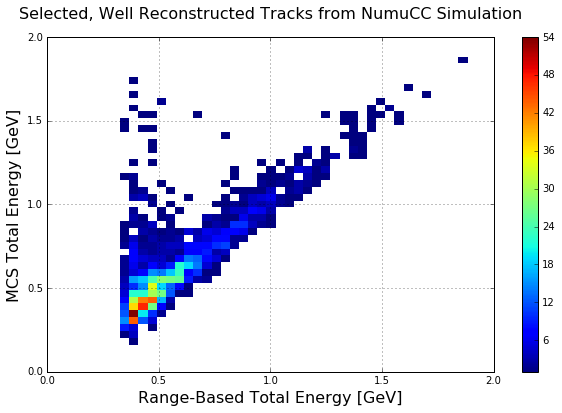
\includegraphics[width=100mm]{Figures/MCS_range_comparison_MCNuRecoTracks_noPDGcut.png}
\end{center}
\caption{\textit{MCS computed energy versus range energy for the selected simulated neutrino-induced fully contained, well reconstructed muon sample without any additional cuts to mitigate MIDs.}}
\label{MCS_range_energy_MCNuRecoTrack_noPDGcut_fig}
\end{figure}

\begin{figure}
\centering
\mbox{
	\subfigure[\textit{The subset of events in Figure \ref{MCS_range_energy_MCNuRecoTrack_noPDGcut_fig} in which the true identity of the track is a proton.}]
	{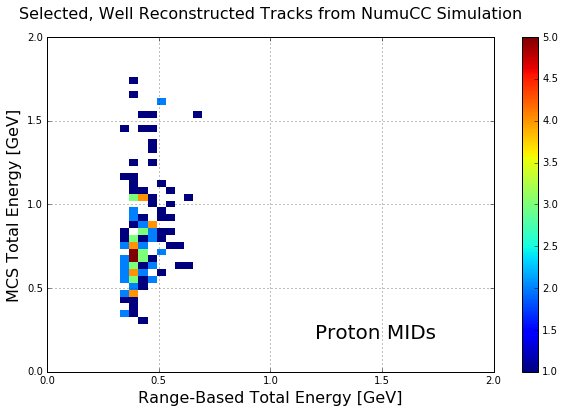
\includegraphics[width=50mm]{Figures/MCS_range_energy_MCNuRecoTracks_proton.png}}
	\quad
	\subfigure[\textit{The subset of events in Figure \ref{MCS_range_energy_MCNuRecoTrack_noPDGcut_fig} in which the true identity of the track is a pion.}]
	{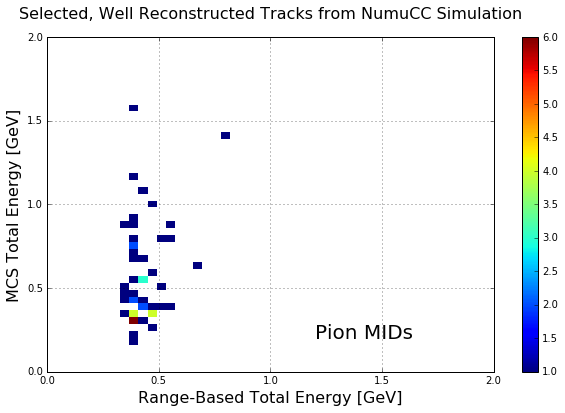
\includegraphics[width=50mm]{Figures/MCS_range_energy_MCNuRecoTracks_pion.png}}
	\quad
	\subfigure[\textit{The subset of events in Figure \ref{MCS_range_energy_MCNuRecoTrack_noPDGcut_fig} in which the true identity of the track is a muon.}\label{MCS_range_energy_MCNuRecoTrack_muononly_fig}]
	{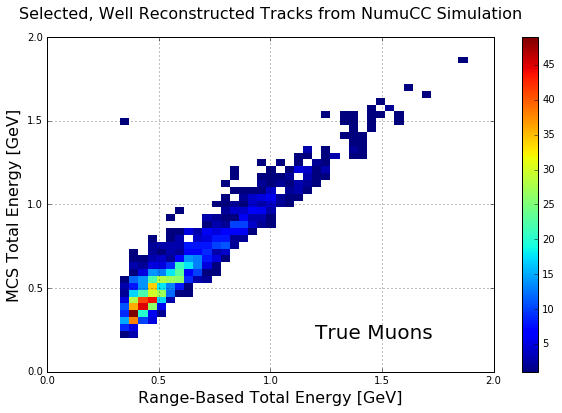
\includegraphics[width=50mm]{Figures/MCS_range_energy_MCNuRecoTracks_muon.png}}
	}
\caption{\textit{MCS computed energy versus range energy for the selected neutrino-induced, well reconstructed fully contained muon sample in simulation broken up by true particle identity of the track.}}
\label{MCS_range_energy_MCNuRecoTrack_withPDGcuts_fig}
\end{figure}


\begin{figure}
\centering
\mbox{
	\subfigure[\textit{Fractional energy difference between 0.35 and 0.53 GeV range energy.}]
	{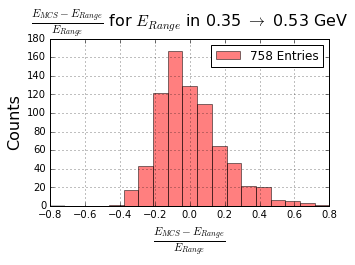
\includegraphics[width=50mm]{Figures/MCS_range_resolution_MCNuRecoTracks_slice1.png}}
	\quad
	\subfigure[\textit{Fractional energy difference between 0.90 and 1.08 GeV range energy.}]
	{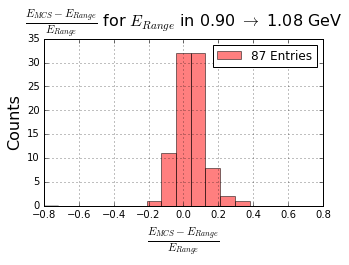
\includegraphics[width=50mm]{Figures/MCS_range_resolution_MCNuRecoTracks_slice2.png}}
	\quad
	\subfigure[\textit{Fractional energy difference between 1.45 and 1.63 GeV range energy.}]
	{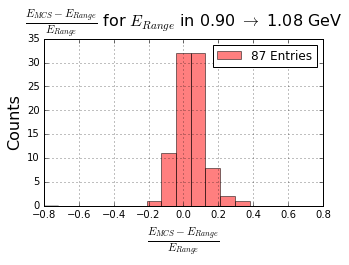
\includegraphics[width=50mm]{Figures/MCS_range_resolution_MCNuRecoTracks_slice2.png}}
	}

\caption{\textit{Fractional energy difference for a few representative bins of range energy derived from Figure \ref{MCS_range_energy_MCNuRecoTrack_muononly_fig}.}}
\label{MCS_range_bias_resolution_MCNuRecoTrack_slices_fig}
\end{figure}


\begin{figure}
\centering
\mbox{
	\subfigure[\textit{MCS energy bias as a function of range energy.}]
	{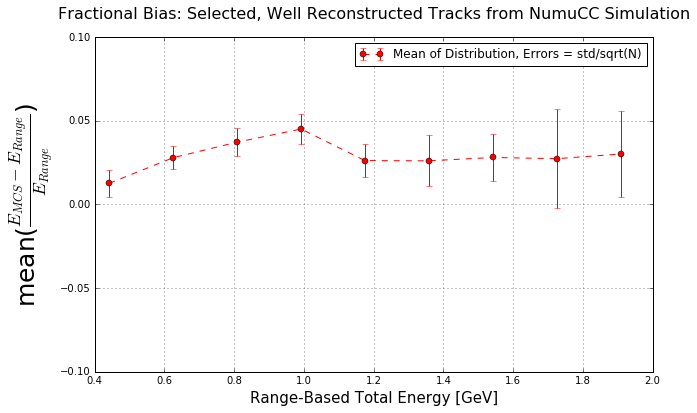
\includegraphics[width=75mm]{Figures/MCS_range_bias_MCNuRecoTracks.png}}
	\quad
	\subfigure[\textit{MCS energy resolution as a function of range energy.}]
	{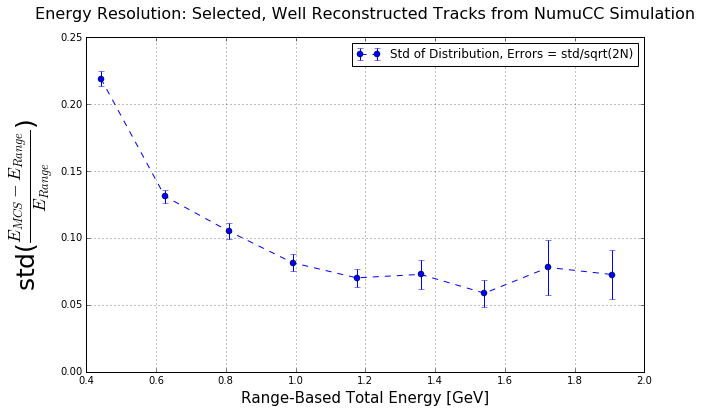
\includegraphics[width=75mm]{Figures/MCS_range_resolution_MCNuRecoTracks.png}}
	}
\caption{\textit{MCS energy bias and resolution as a function of range energy for the selected, well reconstructed neutrino-induced muons in {\ub} simulation.}}
\label{MCS_range_bias_resolution_MCNuRecoTrack_fig}
\end{figure}



\subsection{Highland Validation}\label{Highland_Validation_MCNuRecoTrack_section}
For this sample of contained, selected, well-reconstructed neutrino-induced tracks, the same Highland validation plot is created in exactly the same way as described in Section \ref{Highland_Validation_MCTrack_section}. For each consecutive pairs of segments, the angular scatter in milliradians divided by the Highland expected RMS in millradians is an entry in the histogram shown in Figure \ref{Highland_validation_MCNuRecoTracks_fig}. From this figure we can see that the Highland formula is valid for well reconstructed tracks in data.

\begin{figure}[h!]
\begin{center}
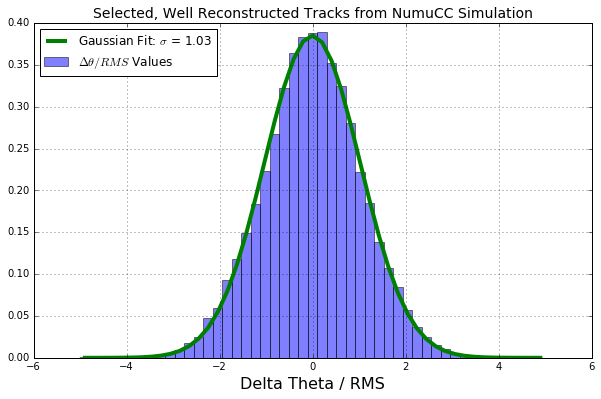
\includegraphics[width=100mm]{Figures/Highland_validation_MCNuRecoTracks_muon.png}
\end{center}
\caption{\textit{20cm segment angular deviations divided by expected Highland RMS for the sample of well reconstructed, neutrino induced muons in simulation.}}
\label{Highland_validation_MCNuRecoTracks_fig}
\end{figure}